\documentclass[aspectratio=169]{beamer}

% Copyright (C) 2012 - EDF R&D - Michael Baudin

% To highlight source code
\usepackage{listings}
\definecolor{darkgreen}{rgb}{0,0.5,0}
\definecolor{violet}{rgb}{0.5,0,1}

% \usepackage{lmodern}% http://ctan.org/pkg/lm

\usetheme{Darmstadt} % http://tex.stackexchange.com/questions/177042/beamer-latex-customized-formats

\useoutertheme[subsection=false,footline=authortitle]{miniframes}
% RGB scaled on 0-255 scale (section 17.1.1), colors pulled from title block
\usecolortheme[RGB={44, 131, 82}]{structure}

% hide header:
\setbeamertemplate{headline}{}

\usepackage[utf8]{inputenc}
\usepackage[T1]{fontenc}

%\usepackage[french]{babel}
%\uselanguage{French}
%\languagepath{French}

\def\bx{{\bf x}}
\def\RR{\mathbb{R}}

% The physical model
\newcommand{\model}{g}
\newcommand{\inputDim}{d}  % The input dimension of the model
\newcommand{\outputDim}{{d_Y}}  % The output dimension of the model
\newcommand{\metaModel}{\widetilde{\model}}  % The surrogate model

% Probabilistic modeling
\newcommand{\inputRV}{\vect{X}}  % The input random vector of the model
\newcommand{\outputRV}{\vect{Y}}  % The output random vector of the model
\newcommand{\inputMeasure}{\mu_{\inputRV}}  % The distribution of the input random vector of the model
\newcommand{\outputMeasure}{\mu_{\outputRV}}  % The distribution of the output random vector of the model
\newcommand{\standardRV}{\vect{Z}}  % The standard random vector (e.g. for polynomial chaos expansion)
\newcommand{\RVU}{\vect{U}}

% For matrixes and vectors
\newcommand{\vect}[1]{{\mathbf{\boldsymbol{{#1}}}}}
\newcommand{\mat}[1]{{\vect{\vect{#1}}}}
\newcommand{\Tr}[1]{{#1}^\top}

% Probabilistic operators
\newcommand{\muX}{\vect{\mu}_{\:X}}
\newcommand{\Var}[1]{{\rm Var}\left( #1 \right)}
\newcommand{\Cov}[1]{{\rm Cov}\left( #1 \right)}
\newcommand{\Expect}[1]{{\mathbb E}\left[ #1 \right]}
\newcommand{\Econd}[2]{{\mathbb E}_{#1}\left[ #2 \right]}
\newcommand{\Prob}[1]{{\mathbb P}\left( #1 \right)}
\newcommand{\ProbCond}[2]{{\mathbb P}_{#1}\left( #2 \right)}
\newcommand{\ech}{\left\{ x_1, \, \dots\,, x_N  \right\}}
\newcommand{\matcov} {\mathbf C}
\newcommand{\matcor} {\mathbf R}
\newcommand{\fcar}[2] {{\mathbf 1}_{#1}(#2)}

\newcommand{\pyvar}[1]{\texttt{#1}}

\def \ot {OpenTURNS}

\hypersetup{colorlinks=true}

\lstset{
  % general command to set parameter(s)
   %basicstyle=\footnotesize\ttfamily, %
   %basicstyle=\normalsize \ttfamily, %
   basicstyle=\scriptsize\ttfamily, %
   keywordstyle=\color{violet}\bfseries,%
   commentstyle=\color{darkgreen}\bfseries,%
   showspaces=false,%
   stringstyle=\color{red}\bfseries, 
   otherkeywords={Gumbel, TruncatedDistribution, LatentVariableModel, %
        SmoothedUniformFactory, Uniform, PythonFunction, JointDistribution, %
        StudentCopula, StudentCopulaFactory, RankSobolSensitivityAlgorithm, %
	   MonteCarlo, IntervalMesher, PointToFieldFunctionalChaosAlgorithm, FieldFunctionalChaosSobolIndices, HistogramFactory, %
	   Graph, BoxCoxFactory, CompositeProcess, WhittleFactory, ARMAFactory, %
	   Basis, TrendFactory, BoxCoxTransform, SpatialFunction, TimeSeries, %
	   WelchFactory, GreaterOrEqual, IndependentCopula, %
	   FunctionalChaosAlgorithm, LowDiscrepancyExperiment, HaltonSequence, LOLAVoronoi,
	   SystemFORM, UnionEvent, IntersectionEvent},
}


\title[OpenTURNS]{OpenTURNS (parts of) release highlights}

\author[OpenTURNS et al.]{M.Baudin (EDF)}

\date[]{User Day \#18, June 13th 2025, EDF Lab}

\titlegraphic{
  
\includegraphics[height=0.04\textheight]{figures/airbus-logo-3d-blue.png} \hfill
  
\includegraphics[height=0.09\textheight]{figures/logo-edf.png} \hfill
  
\includegraphics[height=0.09\textheight]{figures/imacs-logo.jpg} \hfill
  
\includegraphics[height=0.05\textheight]{figures/onera-logo.png} \hfill
  
\includegraphics[height=0.08\textheight]{figures/logo-phimeca.png}
  }

%%%%%%%%%%%%%%%%%%%%%%%%%%%%%%%%%%%%%%%%%%%%%%%%%%%%%%%%%%%%%%%%%%%%%%%%%%%%%

\begin{document}

%%%%%%%%%%%%%%%%%%%%%%%%%%%%%%%%%%%%%%%%%%%%%%%%%%%%%%%%%%%%%%%%%%%%%%%%%%%%%

\begin{frame}
\titlepage

\end{frame}

%%%%%%%%%%%%%%%%%%%%%%%%%%%%%%%%%%%%%%%%%%%%%%%%%%%%%%%%%%%%%%%%%%%%%%%%%%%%%

\begin{frame}
\frametitle{Contents}
\tableofcontents
\end{frame}

%%%%%%%%%%%%%%%%%%%%%%%%%%%%%%%%%%%%%%%%%%%%%%%%%%%%%%%%%%%%%%%%%%%%%%%%%%%%%

\section{QuantileConfidence}

\begin{frame}{QuantileConfidence}

  \emph{Joint work with A. Dutfoy, J.Schueller.}

  \textbf{QuantileConfidence}
  \begin{itemize}
  \item Goal: estimate the confidence interval of a 
  quantile\footnote{See Meeker, W. Q., Hahn, G. J., and Escobar, L. A. (2017). \emph{Statistical intervals: a guide for practitioners and researchers}, volume 541. John Wiley \& Sons.}.
  \item In the nuclear industry, this is called\footnote{See Wilks, S. S. (1941). \emph{Determination of sample sizes for setting tolerance limits.} The Annals of Mathematical Statistics, 12(1), 91-96.} 
  "Wilks's method", but \textbf{this is not proper}, since Wilks's paper 
  introduces a tolerance interval, not a confidence 
  interval (this is different in the bilateral case).
  \end{itemize}

  \begin{center}
    
\includegraphics[width=0.6\textwidth]{figures/Wilks_determination_tolerance_limits.png}
  \end{center}
  
\end{frame}

%%%%%%%%%%%%%%%%%%%%%%%%%%%%%%%%%%%%%%%%%%%%%%%%%%%%%%%%%%%%%%%%%%%%%%%%%%%%%

\begin{frame}{QuantileConfidence}

  \textbf{Features}\footnote{See 
  PR \href{https://github.com/openturns/openturns/pull/2882}{\#2882}.}
  \begin{itemize}
    \item Compute a confidence interval of a quantile from a sample without 
    any hypothesis on the distribution of the sample. Unilateral or bilateral.
    \item Compute the sample size so that the extreme observations of a sample 
    create a confidence interval of a quantile.
    \item Based on \textbf{efficient algorithms}: e.g. no hard-coded upper 
    bounds on the sample size, no iterative algorithm if a special function 
    can be used, etc.
    \item Compute either an \textrm{ot.Interval} or the rank of the order 
    statistics.
    \item Compute an asymptotic bilateral confidence interval.
    \item Many formulas are based on the quantile (or complementary quantile) 
    of level $\beta$ (the     confidence level) of the binomial distribution 
    with parameters $\alpha$ 
    (the quantile level) and $n$ (the sample size).
    \item The \textrm{Wilks} class is deprecated in 1.25.
    \item In OT 1.24: Improves the documentation\footnote{See 
    PR \href{https://github.com/openturns/openturns/pull/2712}{\#2712}.}
  \end{itemize}

\end{frame}

%%%%%%%%%%%%%%%%%%%%%%%%%%%%%%%%%%%%%%%%%%%%%%%%%%%%%%%%%%%%%%%%%%%%%%%%%%%%%

\begin{frame}[fragile]
  \frametitle{QuantileConfidence}
  \textbf{Example.}
  Compute the upper tail confidence interval $\left]-\infty, X_{(k_{up})}\right]$ 
  such that:
  \[
  \mathbb{P}\left( x_{\alpha} \in \left]-\infty, X_{(k_{up})}\right]\right) \geq \beta.
  \]
  \begin{lstlisting}[language=Python]
    import openturns as ot
    import openturns.experimental as otexp
    alpha = 0.05  # The quantile level
    beta = 0.95  # The confidence level
    algo = otexp.QuantileConfidence(alpha, beta)
    # If the size is known
    rank = algo.computeUnilateralRank(100)  # Returns rank = 9 in {0, ..., 99}
    # On a ot.Sample
    sample = ot.Gumbel().getSample(100)
    ci = algo.computeUnilateralConfidenceInterval(sample)
  \end{lstlisting}

  Depending on the value of the parameters, an exception may be produced if 
  the sample size is too small or the confidence level is too close to 1.

\end{frame}
  
%%%%%%%%%%%%%%%%%%%%%%%%%%%%%%%%%%%%%%%%%%%%%%%%%%%%%%%%%%%%%%%%%%%%%%%%%%%%%

\section{otbenchmark}

\begin{frame}{otbenchmark}
  \emph{Joint work with E. Fekhari, M. Baudin, V. Chabridon, Y. Jebroun, 
  J. Schueller.}

  \textbf{otbenchmark}\footnote{See Fekhari, E., Baudin, M., Chabridon, V., 
  \& Jebroun, Y. (2021). 
  \emph{otbenchmark: An open source Python package for benchmarking and 
  validating uncertainty quantification algorithms.} 
  In 4th International Conference on Uncertainty Quantification in 
  Computational Sciences and Engineering.}
  is a benchmark package for Uncertainty Quantification.
  \begin{center}
    \begin{tikzpicture}
      % Place nodes
        \tiny
        \node [mybox1] (0) {\textbf{\pyvar{otbenchmark}}};
        \node [mybox] [right=2mm of 0] (i1) {UQ methods};
        \node [mybox] [left=2mm of 0, align=center] (i3) {benchmark problems \&\\reference values};
        \node [mybox] [below=2mm of 0, align=center] (i2) {performance metrics \&\\graphical tools};
        \node[above=5mm of 0, align=center] (title) {\textcolor{otgreen}{OpenTURNS probabilistic programming paradigm}};
    
        \path[-stealth]
        (i3) edge[very thick, bend left=15] (i1)
        (i1) edge[very thick, bend left=15] (i2)
        (i2) edge[very thick, bend left=15] (i3);
    
      \begin{pgfonlayer}{background} 
        \node[otbox, fit=(i1) (i2) (i3) (title), draw] (Input) {};
        \end{pgfonlayer}
      
      \only{\node [mybox2] [above right=4mm of i1] (i4) {New methods};}
      \path[->] (i4) edge[bend right=10] (0);
    
      \only{\node [mybox2] [below right=4mm of i1] (i5) {New problems};}
      \path[->] (i5) edge[bend left=10] (0);
      \end{tikzpicture}
  \end{center}
\textbf{Use cases:}
  \begin{itemize}
    \item test a \alert{new UQ algorithm} on a panel of problems
    \item compare several UQ algorithms available on a given \alert{benchmark problem}
  \end{itemize}

  
\end{frame}

%%%%%%%%%%%%%%%%%%%%%%%%%%%%%%%%%%%%%%%%%%%%%%%%%%%%%%%%%%%%%%%%%%%%%%%%%%%%%

\begin{frame}{otbenchmark}

  Two categories of benchmark classes are currently provided:
  \begin{itemize}
    \item reliability problems, i.e. estimating the probability that the 
    output of a function is less than a threshold,
    \item sensitivity problems, i.e. estimating sensitivity indices, for 
    example Sobol' indices.
  \end{itemize}

  \textbf{Features:}
  \begin{itemize}
    \item Most of the reliability problems were adapted from the 
    RPRepo\footnote{See Rozsas A., Slobbe A. (2019). Repository and Black-box 
    Reliability Challenge 2019. 
    \url{https://rprepo.readthedocs.io/en/latest/}.}.
    
    \item Create a problem, run an algorithm and compare the computed 
    probability with a reference probability.

    \item Loop over all problems and run several methods on these problems.

    \item \textbf{26 reliability problems} and \textbf{12 sensitivity analysis 
    problems} so far

    \item Reference values either computed by exact quadrature methods or large 
    Monte Carlo sampling.
  \end{itemize}
\end{frame}
  
%%%%%%%%%%%%%%%%%%%%%%%%%%%%%%%%%%%%%%%%%%%%%%%%%%%%%%%%%%%%%%%%%%%%%%%%%%%%%

\begin{frame}[fragile]
  \frametitle{otbenchmark}

  Already presented\footnote{See Fekhari, E., Baudin, M., Chabridon, V., 
  \& Jebroun, Y. (2021, June 9). 
  \emph{OTBenchmark: An open source Python package for benchmarking and 
  validating uncertainty quantification algorithms}. 
  OpenTURNS User's Day 2019. 
  \href{https://github.com/openturns/presentation/blob/master/userday2021/jot_efekhari21.pdf}{jot\_efekhari21.pdf}.} at OpenTURNS User's Day 2019.

  \textbf{New in 2025}: 

  \begin{itemize}
    \item Repo moved into openturns: \url{https://github.com/openturns/otbenchmark}
    \item Online documentation: \url{https://openturns.github.io/otbenchmark/master/}
    \item Conda and pip packaging\footnote{See 
    \href{https://anaconda.org/conda-forge/otbenchmark}{here} and 
    \href{https://pypi.org/project/otbenchmark/}{there}.}:
    \begin{lstlisting}
      conda install otbenchmark  # ... or ....
      pip install otbenchmark
    \end{lstlisting}
  \end{itemize}

  \begin{center}
  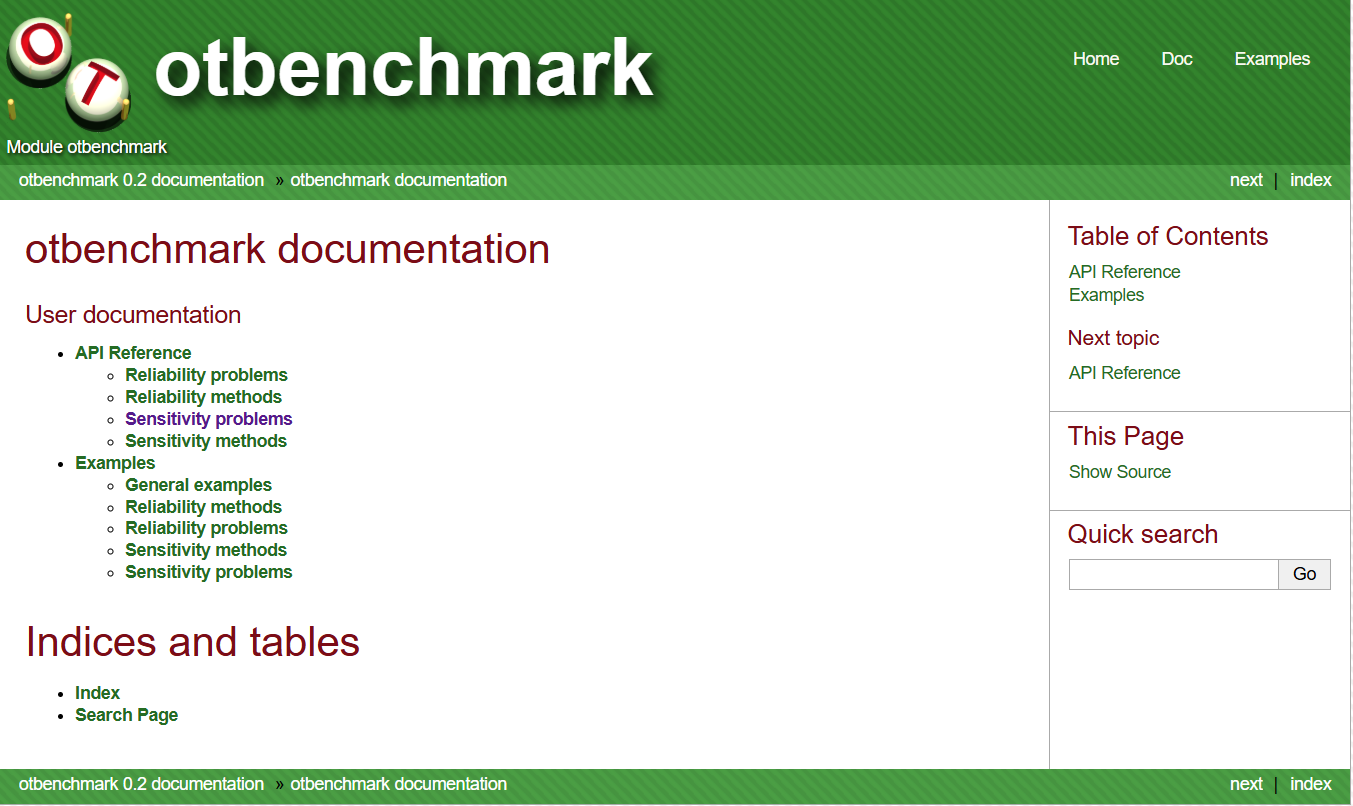
\includegraphics[width=0.3\textwidth]{figures/otbenchmark-help.png}
  \end{center}
\end{frame}

%%%%%%%%%%%%%%%%%%%%%%%%%%%%%%%%%%%%%%%%%%%%%%%%%%%%%%%%%%%%%%%%%%%%%%%%%%%%%

\end{document}
